\newpage

\section*{Локация:}

Все лежит в ауд. 453 на Биржевой. \\

\section*{Характеристики оборудования:}

\begin{itemize}
    \item Автопилот --- Pixhawk 2.4.8 \\
    \begin{itemize}
        Processor: 
        \item 32bit STM32F427 Cortex-M4F core with FPU
        \item 168 MHz
        \item 256 KB RAM
        \item 2 MB Flash
        \item 32 bit STM32F103 failsafe co-processor \\
        
        Sensors:
        \item ST Micro L3GD20H 16 bit gyroscope
        \item ST Micro LSM303D 14 bit accelerometer / magnetometer
        \item Invensense MPU 6000 3-axis accelerometer/gyroscope
        \item MEAS MS5611 barometer \\
        
        Interfaces: 
        \item 5x UART (serial ports), one high-power capable, 2x with HW flow control
        \item 2x CAN (one with internal 3.3V transceiver, one on expansion connector)
        \item Spektrum DSM / DSM2 / DSM-X Satellite compatible input
        \item Futaba S.BUS compatible input and output
        \item PPM sum signal input
        \item RSSI (PWM or voltage) input
        \item I2C
        \item SPI
        \item 3.3 and 6.6V ADC inputs
        \item  Internal microUSB port and external microUSB port extension
    \newpage
    \end{itemize}
    \item Двигатели --- BlueRobotics T200
    \begin{center}
        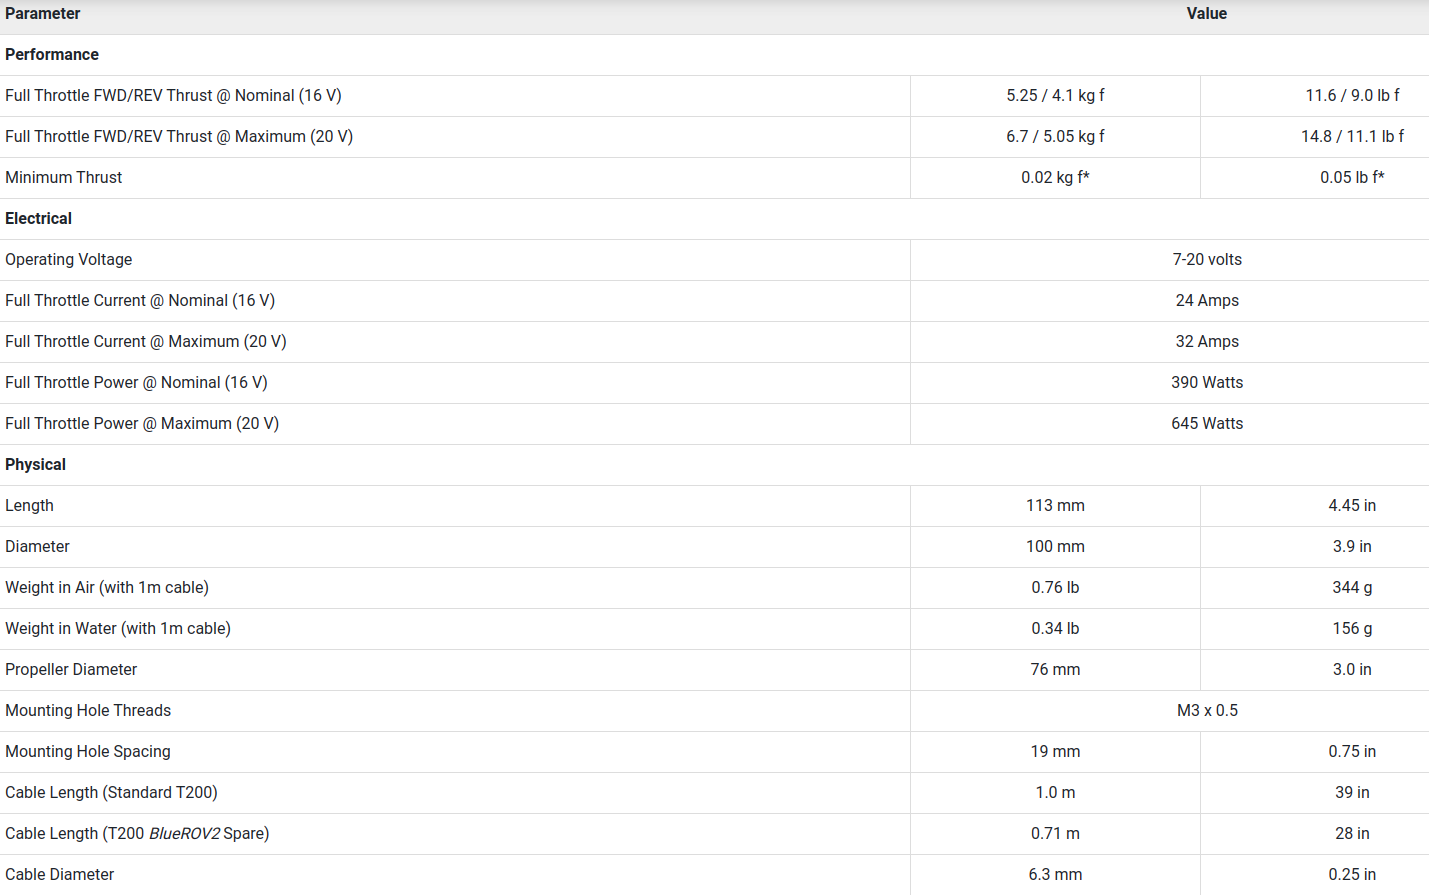
\includegraphics[width=1\textwidth]{img/thrs-table.png}\\
    \end{center} 
    \item Регуляторы скорости --- BlueRobotics
    \begin{center}
        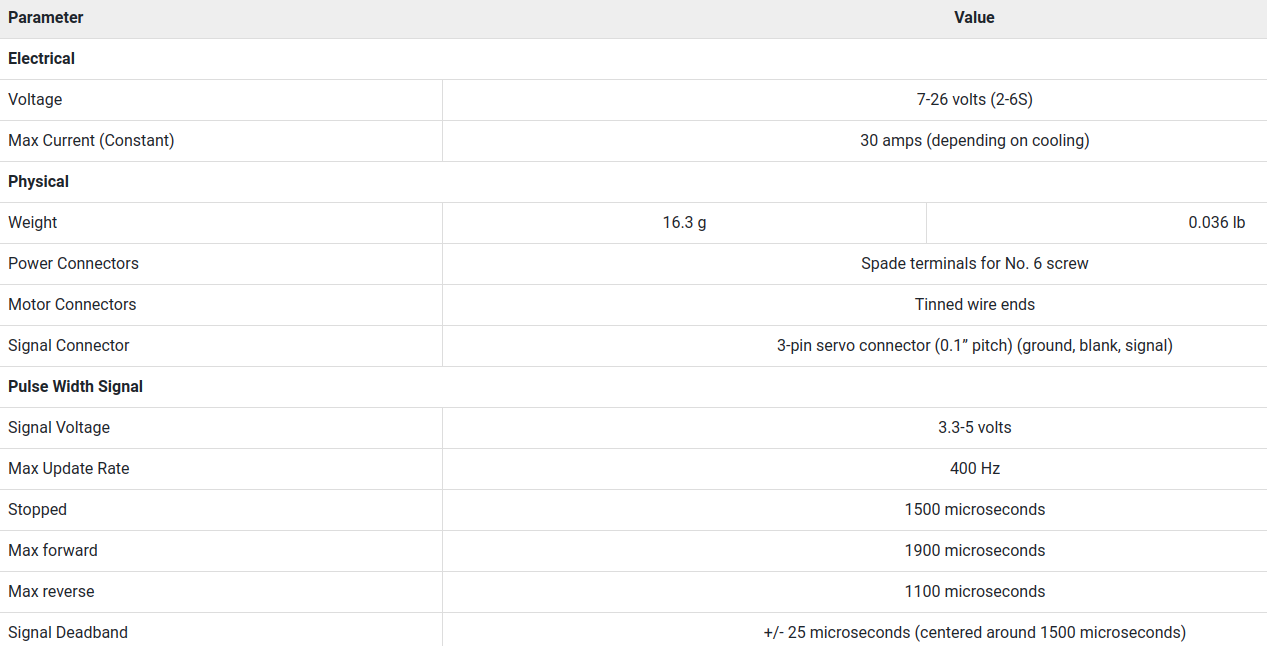
\includegraphics[width=1\textwidth]{img/esc.png}\\
    \end{center} 
    
    \newpage
    \item Микроконтроллер --- Rasberry Pi 4 \\
    \begin{itemize}
        \item Hardware:
        \item Quad core 64-bit ARM-Cortex A72 running at 1.5GHz
        \item 1, 2 and 4 Gigabyte LPDDR4 RAM options
        \item H.265 (HEVC) hardware decode (up to 4Kp60)
        \item H.264 hardware decode (up to 1080p60)
        \item VideoCore VI 3D Graphics
        \item Supports dual HDMI display output up to 4Kp60 \\
        
        Interfaces: 
        \item 802.11 b/g/n/ac Wireless LAN
        \item Bluetooth 5.0 with BLE
        \item 1x SD Card
        \item 2x micro-HDMI ports supporting dual displays up to 4Kp60 resolution
        \item 2x USB2 ports
        \item 2x USB3 ports
        \item 1x Gigabit Ethernet port (supports PoE with add-on PoE HAT)
        \item 1x Raspberry Pi camera port (2-lane MIPI CSI)
        \item 1x Raspberry Pi display port (2-lane MIPI DSI)
        \item 28x user GPIO supporting various interface options:
    \end{itemize}
    \item pH sensor \\
    \begin{itemize}
        \item Sensor type: Combination electrode
        \item Measurement range: 0~14 pH
        \item Temperature of operation: 0~80 ºC
        \item Zero electric potential: 7±0.25 p
        \item Response time: \<1 min
        \item Internal resistance: ≤250 MΩ
        \item Repeatability: 0.017
        \item PTS (percentage of slope ): >98.5
        \item Noise: \<0.5 mV
        \item Alkali error: 15 mV
        \item Reader accuracy: up to 0.01 (in function of calibration)
        \item Cable length: ~500 cm
    \end{itemize}
    \item Temperature sensor: \\
    \begin{itemize}
        \item Measurement range: 0 ~ 100 ºC
        \item Accuracy: DIN EN 60751
        \item Resistance (0 ºC): 1000 Ω
        \item Diameter: 6 mm
        \item Length: 40 mm
        \item Cable length: ~500 cm
    \end{itemize}
    \item Conductivity sensor: \\
    \begin{itemize}
        \item Sensor type: Two electrodes sensor
        \item Electrode material: Platinum
        \item Conductivity cell constant: 1 ± 0.2 ${cm^{-1}}$
        \item Cable length: ~500 cm
    \end{itemize}
    
\end{itemize}

\section*{Вес:}

\begin{itemize}
    \item Лодка с двигателями --- 11000 г
    \item Аккумуляторы --- 2*2100 г
    \item Бокс --- 2240 г
    \item Двигатели --- 2*344 г (на воздухе)
\end{itemize}

\section*{Размеры:}

\begin{center}
        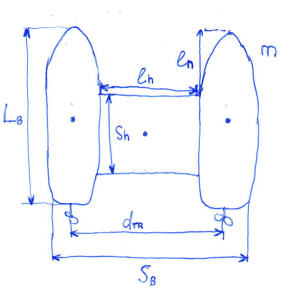
\includegraphics[width=0.6\textwidth]{img/boat-size.png}\\
\end{center} 
    
\begin{eqnarray*}
    L_B = 1100 mm \\
    d_{TR} = 630 mm \\
    S_B = 900 mm \\
    l_n = 420 mm \\
    l_h = 410 mm \\
    S_h = 490 mm
\end{eqnarray*}

\newpage

\section*{Моменты инерции (из Компаса):}

\begin{center}
        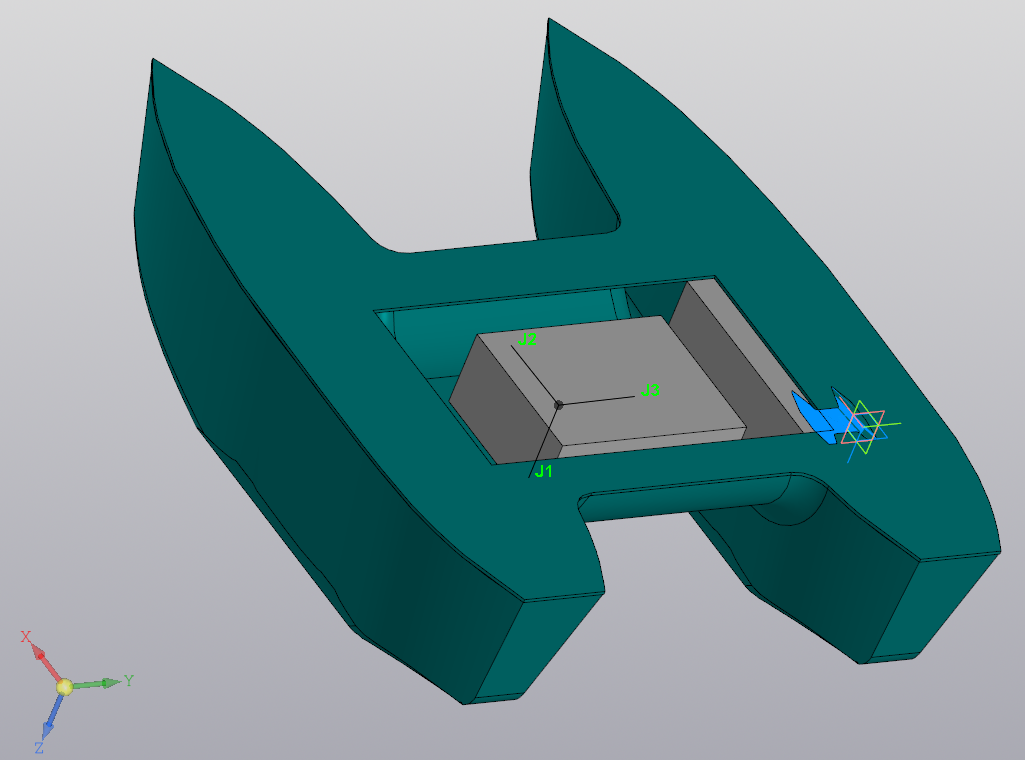
\includegraphics[width=0.6\textwidth]{img/Moments.PNG}\\
\end{center} 

\begin{eqnarray*}
\text{Масса:} \qquad                             M = 17.285092\; kg \\
\text{Площадь:}    \qquad                        S = 4.760588\; m^2 \\
\text{Объем:}   \qquad                           V = 0.032744\; m^3 \\
\text{Центр масс:}  \qquad                      X_c = 0.213901\; m \\
                                  Y_c = -0.320188\; m \\
                                  Z_c = 0.106578\; m \\
\end{eqnarray*}
\text{Осевые моменты инерции:} \\
\begin{eqnarray*}
J_x = 1.695259\; kg*m^2 \\
J_y = 1.073991\; kg*m^2 \\
J_z = 2.522774\; kg*m^2 \\
\end{eqnarray*}
\text{Центробежные моменты инерции:}     \\
\begin{eqnarray*}
J_{xy} = 0.008403\; kg*m^2 \\
J_{xz} = 0.007274\; kg*m^2 \\
J_{yz} = -0.000170\; kg*m^2 \\
\end{eqnarray*}
\text{В главной центральной системе координат:} \\
\begin{eqnarray*}
J_1 = 2.522838\; kg*m^2 \\
J_2 = 1.695309\; kg*m^2 \\
J_3 = 1.073877\; kg*m^2 \\
\end{eqnarray*}
